\section{Teoria e Problema}
\label{sezione2}
\subsection{Introduzione}
Per poter svolgere l'esercizio è necessario capire, anche se brevemente, cosa sono gli Alberi Binari di Ricerca (in generale) e successivamente una comprensione delle sue varianti più "potenti". 
In particolare come tali alberi sono visti come una Struttura Dati e conseguentemente gli eventuali Algoritmi che possono essere utilizzati su di essi.
L'Algoritmo su cui mi soffermerò in maniera approfondita sarà l'algoritmo di inserimento (per ogni tipologia di Albero Binario di Ricerca), in quanto essenziale per la loro creazione, e la sua complessità computazionale. Verrà fatto invece solo un accenno sulla complessità computazionale della ricerca e della cancellazione (senza approfondimento).
\subsection{Notazioni e concetti da usare}
Per trattare i successivi argomenti è necessario usufruire di alcune notazioni della teoria della complessità computazionale, come ad esempio $O(\cdot)$ e $\Theta(\cdot)$. Infine faremo riferimento a \textit{n} come al numero di nodi di un albero ed \textit{h} come la sua altezza. Infine useremo $lg(n)$ = $\log_{2}(n)$ come notazione per il logaritmo in base 2.
\subsection{Cosa è un Albero Binario di Ricerca?}
Gli Alberi Binari di Ricerca (brevemente ABR) sono strutture dati che supportano molte operazioni sugli insiemi dinamici. Gli ABR sono organizzati in alberi binari dove ogni Nodo è visto come un oggetto. Ciascun Nodo possiede pertanto i seguenti campi:
\begin{itemize}
	\item \textit{Key}: la chiave, valore, del nodo in questione più eventuali dati satelliti
	\item \textit{Left}: puntatore al figlio sinistro
	\item \textit{Right}: puntatore al figlio destro
	\item \textit{p}: puntantore al padre.
\end{itemize}
Se manca un figlio o un padre i corrispondenti campi hanno valore \textbf{NIL}. Il nodo Radice \textit{(Root)} è l'unico nodo il cui campo padre \textit{p} è \textbf{NIL}.
\subsection{Proprietà fondamentale di un ABR}
Le chiavi in un ABR sono memorizzate sempre in modo tale da soddisfare la \textbf{\textit{Proprietà fondamentale di un ABR}}:
\begin{tcolorbox} [colback=lightgray!20,%gray background
colframe=black,% black frame colour
arc=3mm, auto outer arc,]
	\textit{Sia x un nodo all'interno di un ABR. Allora:
		\begin{itemize}
			\item se y è un nodo nel sottoalbero sinistro di x allora y.key $<$ x.key
			\item se y è un nodo nel sottoalbero destro di x, allora y.key $\geq$ x.key
		\end{itemize}}
\end{tcolorbox}
Un esempio grafico che rispetti tale proprietà è il seguente:
\begin{figure}[H]
	\centering
	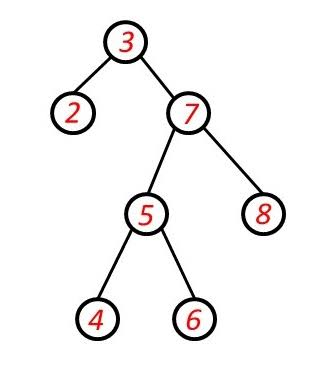
\includegraphics[width=0.3\textwidth]{Resources/ABR_Esempio.jpeg}
	\caption{Esempio di ABR generico}
	\label{fig:immagine}
\end{figure}

\subsection{Altezza di un ABR e Algoritmi Base}
Un fattore molto importante di un ABR, in quanto è una struttura ad albero, è la sua \textbf{altezza}.
 Il costo computazionale per ogni algoritmo utilizzato su tale struttura dati sono determinati da essa.
Algoritmi che di base vengono utilizzati sugli ABR per la manipolazione dei dati sono:
\begin{itemize}
	\item \textbf{Inserimento}
	\item \textbf{Ricerca}
	\item \textbf{Cancellazione}
\end{itemize}
\subsubsection{Inserimento}
L'inserimento di un nodo all'interno dell'ABR viene fatto sfruttando a pieno la proprietà fondamentale di un ABR. Sia pertanto \textit{x} il nodo corrente e sia \textit{z} il nodo da inserire:
\begin{itemize}
	\item la chiave del nodo \textit{z} viene confrontata con la chiave del nodo corrente \textit{x};
	\item in base a tale confronto navigo all'interno dell'albero o a sinistra oppure a destra (in base all'esito del confronto);
	\item la navigazione termina quando \textit{x=NIL}, ovvero sia \textit{x} punta ad una Foglia dell'albero.
\end{itemize}
\subsubsection{Ricerca e Cancellazione}
Ai fini della relazione tratterò solamente i Costi Computazionali a confronto con AVL e RB per la ricerca e cancellazione. Non mi soffermo, in questa sezione, sugli algoritmi di tali metodi.
\subsection{Costo Computazionale}
Per un albero ABR generale la complessità computazionale di un algoritmo di Ricerca, Inserimento o Cancellazione è $\mathcal{O}(h)$ , dove $h$ è l'altezza dell'albero.
Nel caso medio, assumendo che le chiavi siano inserite in ordine
casuale, l'altezza attesa dell'ABR è $\Theta(lg(n))$.
Si distinguono però per l'\textbf{Inserimento} due casi particolari molto importanti:
\begin{itemize}
	\item \textbf{Caso Migliore}: in questa situazione l'altezza dell'albero è circa $\Theta(lg(n))$. Difatti considerando l'albero con questa altezza, per un nodo da inserire, l'inserimento ha complessità computazionale di $\mathcal{O}(\lg(n))$. Questo perchè il confronto della chiave del nodo da inserire non viene fatto con tutti i nodi già presenti all'interno dell'albero in quanto l'albero stesso è "bilanciato" (ovvero sia l'albero presenta in maniera "più o meno simile" il numero di nodi sia a destra che a sinistra prendendo un qualunque nodo come riferimento);
	\item \textbf{Caso Peggiore}: l'albero degenera in una lista. In questa situazione l'altezza dell'albero è circa $\Theta(n)$. Questo avviene quando si ha un inserimento "contiguo" o tutto a sinistra o tutto a destra dell'albero, ovvero sia quando l'inserimento avviene per valori in ordine crescente o decrescente. In questo caso il costo per un singolo inserimento è pari a $\mathcal{O}(n)$.
\end{itemize}
Si ricorda che per un ABR generico, senza proprietà aggiunte, non è presente un ribilanciamento dell'albero.
\subsection{RB e AVL}
Come anticipato esistono delle varianti più potenti di ABR: gli AVL e i RB. Sono varianti che introducono delle proprietà nuove che permettono all'albero un ribilanciamento (in base alle specifiche proprietà) che permettono di abbattere i costi computazionali e di evitare una degenerazione come nel caso dell'inserimento per un ABR generico. Vediamo quindi brevemente le nuove proprietà introdotte e come le due tipologie di varianti riescono a gestire, in particolare per l'inserimento, un ribilanciamento dell'albero binario di ricerca con il fine di abbassare la complessità computazionale.
Per entrambe le varianti si introducono \textbf{Algoritmi di Rotazione Left/Right}, utili per ribilanciare la struttura (più ricolorazioni per gli alberi Rosso-Neri).
\subsubsection{AVL}
Un albero AVL è un albero ABR che si mantiene bilanciato dopo gli inserimenti (e cancellazioni). La proprietà aggiuntiva che viene introdotta è la seguente: 
\begin{tcolorbox} [colback=lightgray!20,%gray background
	colframe=black,% black frame colour
	arc=3mm, auto outer arc,]
	\centering{\textit{Per ogni nodo dell'albero vale} $|h_{sinistro} - h_{destro}| \leq 1$}
\end{tcolorbox}
La nuova regola introdotta ci dice che, in ogni nodo, l'altezza del sottoalbero sinistro e destro può differire al massimo di 1. Se tale proprietà viene violata, l'AVL esegue rotazioni per ribilanciare localmente la struttura. Questo ci garantisce che l'altezza dell'albero è $\Theta(\lg(n))$ e pertanto inserimento, ricerca e cancellazione hanno un costo $\mathcal{O}(\lg(n))$. Si deduce appunto che il caso peggiore visto da un ABR generico viene tranquillamente risolto tramite gli AVL.
\subsubsection{RB}
Un albero Rosso-Nero (\texttt{Red-Black [RB]}) è un ABR auto-bilanciato: per ogni nodo si introduce un colore che può essere rosso oppure nero. Le principali (e quindi nuove) proprietà introdotte sono:
\begin{itemize}
	\item La radice è nera.
	\item Le foglie \textbf{NIL} sono nere.
	\item Un nodo rosso non può avere figli rossi.
	\item Ogni cammino da un nodo a una foglia \textbf{NIL} contiene il medesimo numero di nodi neri.
\end{itemize}
Con queste nuove proprietà si impedisce che l'albero diventi troppo sbilanciato e pertanto dopo inserimenti o cancellazioni, vengono usate ricolorazione dei nodi e rotazioni per ribilanciare localmente la struttura. Come gli AVL, i RB garantiscono altezza $\Theta(lg(n))$ e pertanto per metodi di inserimento e cancellazione il costo computazionale è $\mathcal{O}(lg(n))$. Come nel caso precedente si deduce che il caso peggiore visto da un ABR generico viene tranquillamente risolto anche tramite i RB.
\subsection{Una prima conclusione: assunti ed ipotesi}
\label{Sezione2.8}
Nella \hyperref[sezione2]{Sezione 2} abbiamo affrontato la parte teorica per fare fronte agli esperimenti condotti. Per gli esperimenti affronteremo due casi particolari di costruzioni di alberi binari di ricerca e sue varianti come segue:
\begin{itemize}
	\item \textbf{Caso 1:}  Vengono inserite chiavi distinte in un ordine
	casuale [\textit{Caso medio}]
	\item \textbf{Caso 2:} Vengono inserite chiavi distinte in ordine
	strettamente crescente (o decrescente). L'ABR generico degenera,
	mentre AVL e RB mantengono il bilanciamento [\textit{Caso peggiore per ABR generico}].
\end{itemize}
Le \hyperref[Tabelle2.9]{Tabelle in 2.9} ci permettono di avere un primo confronto tra le diverse strutture dati usate e come l'algoritmo dell'Inserimento si distingue, in termini di costi computazionali, tra le 3 tipologie di ABR per entrambe le casistiche. L'obbiettivo è pertanto quello di verificare che i risultati attesi delle complessità computazionali siano veritieri attraverso la sperimentazione.
\subsection{Tabella delle complessità computazionali a confronto}
Le tabelle seguenti presentano i risultati attesi da verificare successivamente sperimentalmente: ricerca e cancellazione sono riportate come confronto teorico (un approfondimento verrà fatto nella \hyperref[Sezione5.2]{Sezione 5.2}); la sperimentazione considera solamente il costo di costruzione mediante l'inserimento. Per ciascuno dei 2 esperimenti verranno introdotti \textit{x} nodi, sia per il caso randomico e sia per il caso peggiore. Riportiamo in ogni caso il costo computazionale per una singola operazione tra inserimento, ricerca e cancellazione. Si faccia riferimento alla \hyperref[Sezione2.8]{Sezione 2.8} per "Caso 1" e "Caso 2":
\label{Tabelle2.9}
\begin{figure}[H]
	\centering
	\begin{tabular}{|c|c|c|}
		\hline
		& Caso 1 & Caso 2\\
		\hline
		\textcolor{blue}{Inserimento} & $O(lg(n))$ & $O(n)$\\
		\hline
		Ricerca & $O(lg(n))$ & $O(n)$\\
		\hline
		Cancellazione & $O(lg(n))$ & $O(n)$\\
		\hline
	\end{tabular}
	\caption{Complessità degli algoritmi di ABR}
	\label{fig:ComplessitàABR}
\end{figure}

\begin{figure}[H]
	\centering
	\begin{tabular}{|c|c|c|}
		\hline
		& Caso 1 & Caso 2\\
		\hline
		\textcolor{blue}{Inserimento} & $O(lg(n))$ & $O(lg(n))$\\
		\hline
		Ricerca & $O(lg(n))$ & $O(lg(n))$\\
		\hline
		Cancellazione & $O(lg(n))$ & $O(lg(n))$\\
		\hline
	\end{tabular}
	\caption{Complessità degli algoritmi di AVL e RB}
	\label{fig:ComplessitàAVL}
\end{figure}